\documentclass[draftspec]{sbmlpkgspec}
\usepackage{tabularx}

\begin{document}

\packageTitle{The Distributions and Ranges Package\\for SBML Level 3}
\packageVersion{Version 0.5 (Draft)}
\packageVersionDate{6 January, 2012}
%\packageGeneralURL{http://sbml.org/Community/Wiki/SBML_Level_3_Proposals/Distributions_and_Ranges}
%\packageThisVersionURL{}

\author{%
  \begin{tabular}{c>{\hspace{20pt}}c}
    \multicolumn{2}{c}{\Large\bf{Authors}}\\\\
    Stuart L Moodie&Darren Wilkinson\\
    \mailto{moodie@ebi.ac.uk}&\mailto{darren.wilkinson@ncl.ac.uk}\\
    EMBL-EBI& University of Newcastle\\
    Hinxton, UK& Newcastle, UK\\
   \\
    Nicolas Le Nov\`{e}re\\
    \mailto{lenov@ebi.ac.uk}\\
    EMBL-EBI\\
     Hinxton, UK\\\\
    \multicolumn{2}{c}{\Large\bf{Contributors}}\\\\
     \multicolumn{2}{c}{ Colin Gillespie}\\
     \multicolumn{2}{c}{\mailto{c.gillespie@ncl.ac.uk}}\\
     \multicolumn{2}{c}{University of Newcastle}\\
     \multicolumn{2}{c}{ Newcastle, UK}\\
\end{tabular}
}

\notice{Disclaimer: This is a working draft of the SBML Level 3
  ``distib'' package proposal. It is not a normative document.  Please
  send comments and other feedback to the mailing list:
  \mailto{sbml-distrib@lists.sourceforge.net.}}

\maketitlepage
\maketableofcontents

\newcommand\distribshort{distrib\xspace}
\newcommand\distrib{Distributions and Ranges\xspace}
\newcommand\uncertml{UncertML\xspace}
\newcommand\unidistrib{\abstractclass{IUncertainty}\xspace}
\newcommand\mlambda{\class{Lambda}\xspace}
\newcommand\mmath{\class{Math}\xspace}
\newcommand\Distribution{\defRef{Distribution}{sec:distribution}}
\newcommand{\mathml}{MathML\xspace}

\reversemarginpar  % Want "\watchout" to be put on the left, not the right.
\newcommand{\watchout}{\marginpar{\hspace*{34pt}\raisebox{-0.5ex}{\Large\ding{43}}}}
\newcommand{\contraversial}{\marginpar{\hspace*{34pt}\raisebox{-0.5ex}{\Large?}}}

\section*{Revision History}

\begin{edtable}{tabularx}{\linewidth}{c c c X }\toprule
\textbf{Version} & \textbf{Date} & \textbf{Author} & \textbf{Comments} \\ \midrule
0.1 (Draft) & 15 Oct 2011 & Stuart Moodie & First draft \\ \midrule
0.2 (Draft) & 16 Oct 2011 & Stuart Moodie & Added introductory text
and background info. Other minor changes etc. \\ \midrule
0.3 (Draft) & 16 Oct 2011 & Stuart Moodie & Filled empty invocation
semantics section.\\ \midrule
0.4 (Draft) & 4 Jan 2012 & Stuart Moodie & Incorporated comments from
NlN, MS and SK. Some minor revisions and corrections.\\  \midrule
0.5 (Draft) & 6 Jan 2012 & Stuart Moodie & Incorporated addition
comments on aim of package from NlN.\\ 
\bottomrule
\end{edtable}

\section{Introduction and motivation}

\subsection{What is it?}

The \distrib package provides an extension to SBML Level 3 that
supports models that supports variables that cab take many values, for
instance random variables obtained from a statistical
distribution. Applications of the package include for instance
descriptions of the alternative values based on prior knowledge (e.g.\,
experiments), encoding of uncertainty of value and mostly statistical
model or models that require the use of random values, such as PK/PD
models.

% Even in the context of deterministic simulations, it is sometimes
% useful to describe the sampling of a random number during
% simulation. One example is that of a cell dividing once it has grown
% to a given volume. It would be more realistic to initialise species
% concentrations in the resultant daughter cell with random numbers to
% reflect stochastic segragation of proteins, than to have a wholly
% deterministic segregation.

\subsection{This Document}

This proposal presents ideas for the \distrib package proposal, also
``colloquially'' referred to by SBML developers as the \distribshort
package. This is an early draft of the proposal and there are still
many issues to be resolved. In its current state this document aims to
establish a consensus about what has been agreed and what work remains
to be carried out to complete the definition of this package.

This proposal is a working document and should be regarded as a first
step towards the formal adoption of the \distribshort as a package in
SBML Level 3. Later versions of this document will aim to record the
details of the package specification as they evolve, and it will
ultimately serve as a basis for a vote on its adoption by the SBML
community and be the basis for a future package specification
document. More details of the SBML package adoption process can be
found at: \url{http://sbml.org/Documents/SBML_Development_Process}.

\subsection{Conventions used in this document}

As we are early in the package proposal process there will be some
parts of this proposal where there is no clear consensus on the
correct solution or only recent agreement or agreement by a group
which may not be representative of the SBML community as a
whole. These cases are indicated by the \contraversial question mark
in the left margin (illustrated). The reader should pay particular attention to these
points and ideally provide feedback, especially if they disagree with
what is proposed. Similarly there will be points --- especially as the
proposal is consolidated --- which are agreed, but which the reader
should take note of and perhaps read again. These points \watchout are
emphasised by the hand pointer in the left margin (illustrated),

\section{Background}

\subsection{Problems with current SBML approaches}

SBML Level 3 Core has no direct support for providing random values
within a model. Currently there is no workaround and this makes it
impossible to describe models that use probability distributions.

\subsection{Past work on this problem or similar topics}

\subsubsection{The Newcastle Proposal}
\label{sec:newcastle proposal}

In 2005 there was a proposal from Colin Gillespie and others
\footnote{\url{http://sbml.org/Community/Wiki/SBML_Level_3_Proposals/Distributions_and_Ranges}}
to introduce support for probability distributions in the SBML core specification. This
was based on their need to use such distributions to represent the
models they were creating as part of the BASIS project
\url{http://www.basis.ncl.ac.uk}).

They proposed that distributions could be referred to in SBML using
the \class{csymbol} element in the \mathml subset used by
the SBML Core specification. An example is below:

\begin{example}
<xmlns=''http://www.w3.org/1998/Math/MathML''>
  <apply>
    <csymbol encoding=''text''
        definitionURL=''http://www.sbml.org/sbml/symbols/uniformRandom''>
      uniformRandom
    </csymbol>
    <ci>mu</ci>
    <ci>sigma</ci>
  </apply>
</math>
\end{example}

This required that a library of definitions be maintained as part of
the SBML standard and in their proposal they defined an initial small
set of commonly used distributions. The proposal was never
implemented.

\subsubsection{Seattle 2010}

The ``distrib'' package was discussed at the Seattle SBML Hackathon%
\footnote{\url{http://sbml.org/Events/Hackathons/The_2010_SBML-BioModels.net_Hackathon}}. There
one of the authors (DW) presented an overview of the problem%
\footnote{Slides:
 \url{http://sbml.org/images/3/3b/Djw-sbml-hackathon-2010-05-04.pdf}}%
\footnote{Audio:
  \url{http://sbml.org/images/6/67/Wilkinson-distributions-2010-05-04.mov}},
building on the old proposal from the Newcastle group
 (see above: \ref{sec:newcastle proposal}).
There was broad support at the meeting for development of such a
package, and for the proposed feature set. Discussion following the
presentation led to a consensus on the following points:

\begin{itemize}
\item There is an urgent need for such a package.
\item It is important to make a distinction between a description of
  uncertainty regarding a model parameter and the mechanistic process
  of selecting a random number from a probability distribution, for
  applications such as parameter scans and experimental design
\item It is probably worth including the definition of PMFs, PDFs and CDFs in the package
\item It is worth including the definition of random distributions using particle representations within such a package, though some work
 still needs to be done on the precise representation
\item It could be worth exploring the use of xinclude to point at particle
representations held in a separate file
\item Random numbers must not be used in rate laws or anywhere else that
 is continuously evaluated, as then simulation behaviour is not
 defined
\item Although there is a need for a package for describing extrinsic
 noise via stochastic differential equations in SBML, such mechanisms
 should not be included in this package due to the considerable
 implications for simulator developers
\item We probably don't want to layer on top of UncertML
 (www.uncertml.org), as this spec is fairly heavy-weight, and
 somewhat tangential to our requirements
\item A random number seed is not part of a model and should not be
 included in the package
\item The definition of truncated distributions and the specification of
 hard upper and lower bounds on random quantities should be
 considered.
\end{itemize}

It was suggested that new constructs should be introduced into SBML by
the package embedded as user-defined functions using the following
syntax:

\begin{example}
<listOfFunctionDefinitions>
  <functionDefinition id="myNormRand">
    <distrib:####>
      #### distrib binding information here ####
    </distrib:####>
    <math>
      <lambda>
        <bvar>
          <ci>mu</ci>
          <ci>sigma</ci>
        </bvar>
        <ci>mu</ci>
      </lambda>
    </math>
  </functionDefinition>
</listOfFunctionDefinitions>
\end{example}

which allows the use of a "default value" by simulators which do not
understand the package (but simulators which do will ignore the <math>
element). The package would nevertheless be "required", as it will not
be simulated correctly by software which does not understand the
package.

Informal discussions following the break-out covered topics such as
how to work with vector random quantities in the absence of the vector
element in the MathML subset used by SBML, and the care that must be
taken with the semantics of random variables and the need to both a)
reference multiple independent random quantities at a given time and
b) make multiple references to the same random quantity at a given
time.

\subsubsection{Hinxton 2011}

Detailed discussion was continued at the Statistical Models Workshop
in Hinxton in June 2011%
\footnote{\url{http://sbml.org/Events/Other_Events/statistical_models_workshop_2011}}. There
those interested in representing Statistical Models in SBML came
together to work out the details of how this package would work in
detail. Dan Cornford from the \uncertml
project\footnote{\url{http://www.uncertml.org/}} attended the meeting
and described how that resource could be used to describe uncertainty
and in particular probability distributions. Perhaps the most
significant decision at this meeting was to adopt the \uncertml
resource as a controlled vocabulary that is referenced by the \distrib package.

Much of the detail and the examples in this proposal are based on
the work of this workshop and so its outcomes are essentially
presented below. However, at the end of the meeting there remained a
number of unresolved issues that are still unresolved in this
proposal. See section \vref{sec:hinxtonunresolved} for more details.

\section{Proposed syntax and semantics}

\subsection{Colour Conventions}

Throughout this document, in all UML diagrams, classes that exists in
SBML Level 3 core or another existing standard are displayed in
black. If those elements are extended in this proposal, those
extensions are displayed in green. Classes that are new to this
proposal are shown in blue.

\subsection{Defining Distributions}

The \distrib package has a very simple purpose. It defines a
statistical distribution, range or statistic from which you can obtain
a value that is used in other parts of an SBML model. The distribution
is defined using \uncertml, which is a resource that defines
probabilistic uncertainties~\cite{uncertml}, or explicitly using
MathML~\cite{mathml2}.

SBML Core is extended at the \FunctionDefinition class as can be seen
in the UML representation in figure \vref{fig:umlmodel}. The extended
\FunctionDefinition can optionally contain a single instance of a new
class \class{Distribution} that is part of the distrib package. The \class{Distribution} class can
then either refer to an element in UncertML using or alternatively a
\class{Distribution} can contain a \mmath class that is used to define the
distribution explicitly.

\begin{figure}[htb]
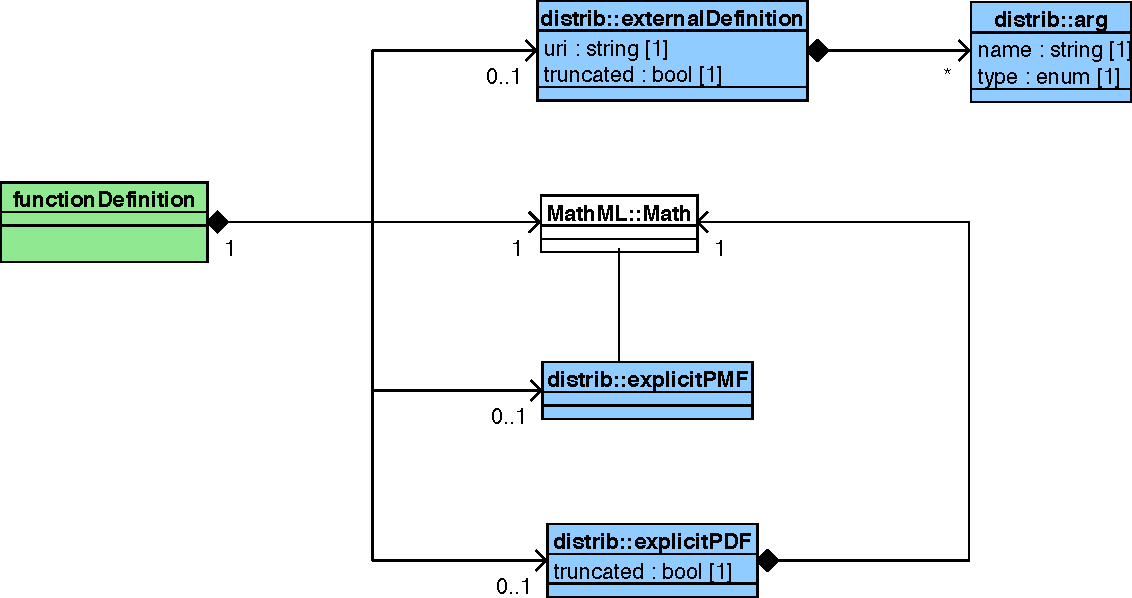
\includegraphics[width=1.0\linewidth]{DistribUMLModel.pdf}
\caption{UML class diagram for the \distrib package. This diagram describes the
  classes involved and not instances of those classes. Note the UML packages
  indicate that the classes belong to different namespaces. The
  namespace of the SBML Core is not shown.}
\label{fig:umlmodel}
\end{figure}

\subsection{Extension Handling}

The \distrib package is defined as a required package, which means
that an SBML model that uses that extension will not be correctly
defined unless the features of the extension are used and interpreted
correctly by supporting software.

\subsection{FunctionDefinition Extension}

As outlined above the \FunctionDefinition is extended to include the
\Distribution class. When \FunctionDefinition contains an instance of
\Distribution this instance must also be accompanied \watchout by an
instance of \mmath that contains \mlambda (see figure
\ref{fig:umluncertmldistrib}). This enables software that cannot understand the
extension to fallback to the \mlambda definition of the function and
so ensure that the SBML representation is self-consistent without the
extension features. We refer to it as the \emph{fallback lambda
  function}.  The fallback lambda function must contain the same
number of input parmeters as the equivalent distribution defined
within \Distribution.

\subsection{Distribution}
\label{sec:distribution}

The \class{Distribution} class contains either an instance of
\unidistrib from \uncertml (figure \ref{fig:umluncertmldistrib}) or an
instance of \mlambda (figure \ref{fig:umlexplicitdistrib}). These instances
are mutually exclusive so only one instance of one type is
permitted. The former form is used when we are referring to an
element define by \uncertml.

\begin{figure}[htb]
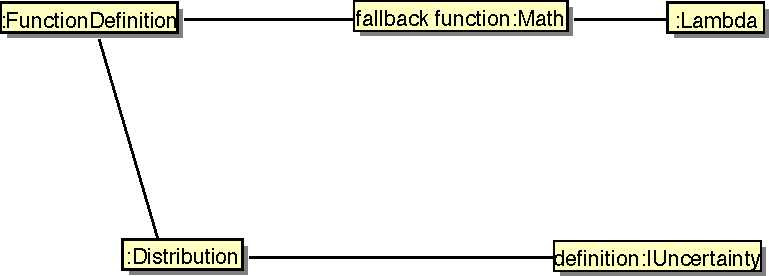
\includegraphics[width=0.7\linewidth]{uncertmlDistrib.pdf}
\caption{UML object diagram describing the definition of a
  distribution using\uncertml.}
\label{fig:umluncertmldistrib}
\end{figure}
 
In this case a \unidistrib is used to reference a distribution defined
by \uncertml. In the explicit form \mathml is used to define a lambda
function that explicitly defines the distribution.
 

\begin{figure}[htb]
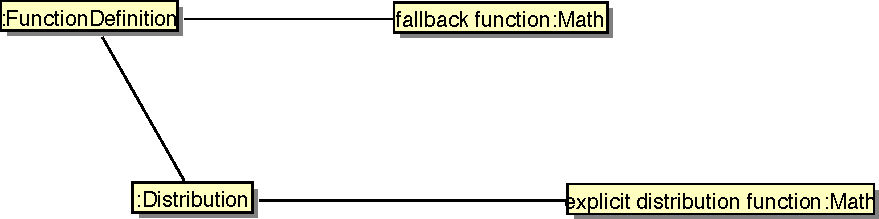
\includegraphics[width=0.7\linewidth]{explicitDistrib.pdf}
\caption{UML object diagram describing the explicit definition of a distribution.}
\label{fig:umlexplicitdistrib}
\end{figure}
 
 The \mathml used in \mlambda is restricted to the same subset as used
in SBML Core. The reader should refer to the SBML Level 3 Core
specification document for more details~\cite{l3v1c}.

\subsection{Attributes}

Here we define the attributes used by the \Distribution class. Each
attribute will have a primitive type and will be always required
(mandatory) or not (optional).

\paragraph{\token{mandatoryEvalRuntime}}

This attribute is a \primtype{boolean} and is required. If its value is \val{true}
then this indicates that the uncertainty is intrinsic to the
model. There is no selection of given values prior to simulation or
analysis. Values are generated during simulation as needed. For
example, a noisy measurement from which any particular value would
lead to a bias and there is no reason to select a particular value,
or white noise where at each realisation, we (may) get a different value.

If the attribute's value is \val{false}, then the uncertainty may be
resolved before simulation. The generation of initial conditions from
the distribution is described in SED-ML. One can choose for instance
to use the mean, or to do a sampling (e.g. parameter scan, random
sampling). For example, a measured parameter for which there are two
different values, or a parameter following a distribution from which
to draw individuals prior to simulation.

\paragraph{\token{truncated}}

This attribute is of type \primtype{boolean} and is required. It
indicates that the distribution is being used only between a given
range and that the attributes \token{lowerBound} and
\token{upperBound} must be set when this instance is invoked.

\paragraph{\token{lowerBound}}

This value is of type \primtype{double} and is not required. It
defines the lower bounds of range within which this distribution will
be used.

\paragraph{\token{upperBound}}

This value is of type \primtype{double} and is not required. It
defines the upper bounds of a range within which this distribution will
be used.

\subsection{Use of \uncertml Definitions}

The abstract class \unidistrib is the super-class of the
distributions,samples and statistics defined by \uncertml. The
appropriate concrete sub-class from \uncertml should be selected and
the appropriate parameters supplied for the distribution. A selection
of \uncertml classes is shown in figure~\vref{fig:ucmldistribs}.

\begin{figure}[htb]
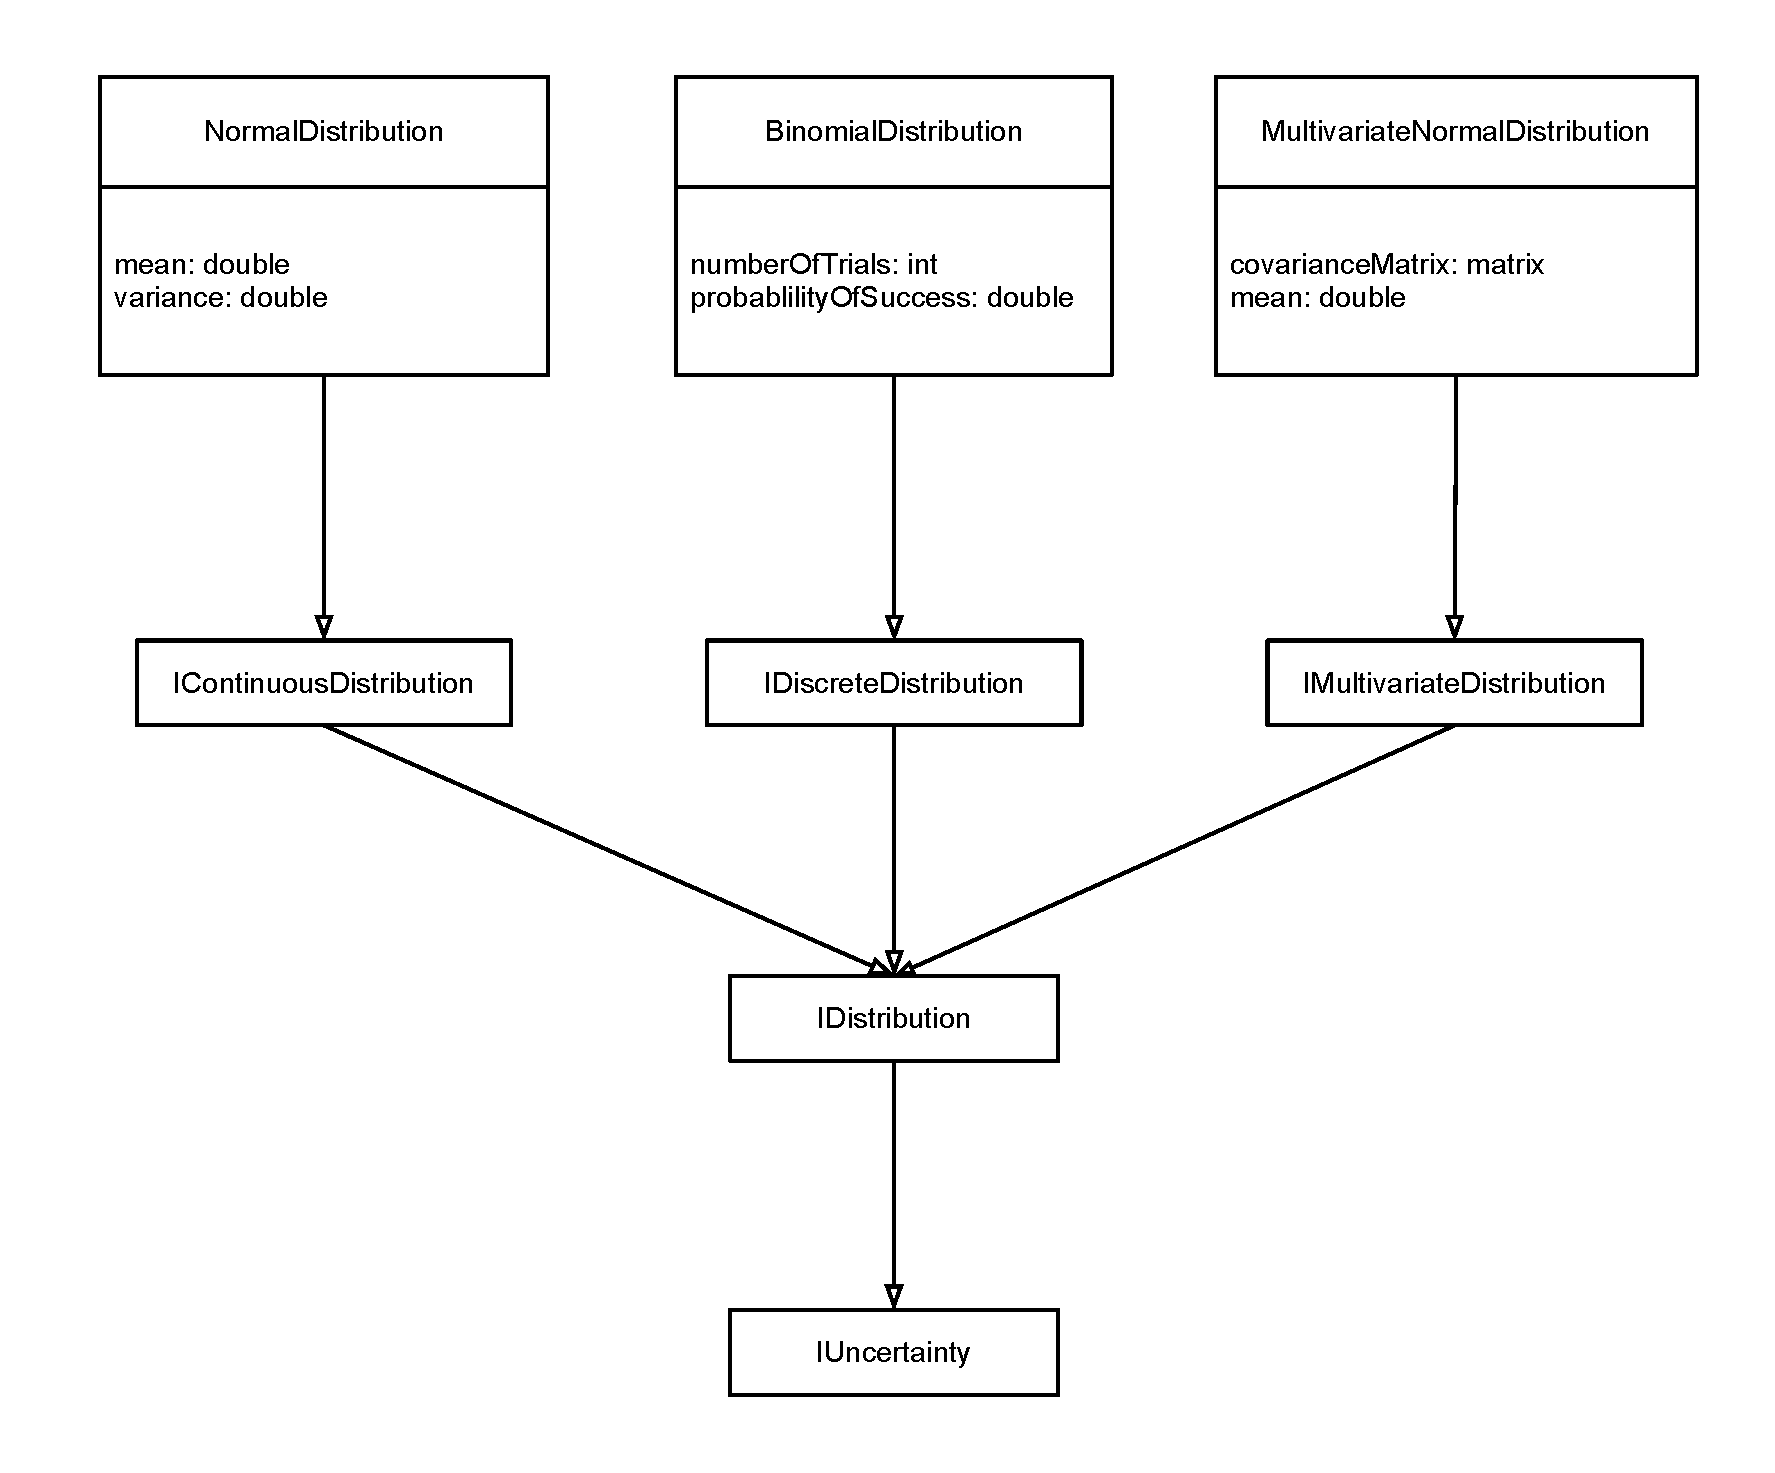
\includegraphics[height=0.5\linewidth]{UncertMLDistributions.pdf}
\caption{A selection of the distributions in \uncertml represented as a UML model.}
\label{fig:ucmldistribs}
\end{figure}

Note \contraversial that to satisfy \uncertml the attributes of a given
distribution class must be supplied with a value. These values act as
a placeholder and must be of the correct type. Some \uncertml
distributions may require an array or a matrix of values as an
attribute.

\subsection{Referencing the \distrib package}

The distribution defined by a \Distribution instance is defined by the
name of its owning \FunctionDefinition instance. Therefore other \SBML
elements can reference a distribution as a function in the same way that they
reference other instances of \FunctionDefinition. The arguments to the function
should match those defined within the \Distribution instance.

\paragraph{Scalar Assumption}

It is assumed \contraversial that all the \uncertml classes will enable
the retrieval of a scalar result of type \primtype{double}. Note that
some \uncertml classes, for example
\class{Range}\footnote{\url{http://www.uncertml.org/statistics/range}}
currently return an array of values. This is an inconsistency that
needs to be resolved.

\paragraph{Type Consistency}

When invoking a \FunctionDefinition that contains a \Distribution
instance one must ensure that the value types are consistent. When the
distribution is defined by a concrete sub-class of \unidistrib the
paramaters used in the function call must match those defined in the
\uncertml class specification. For example the
\class{PoissonDistribution}\footnote{http://www.uncertml.org/distributions/poisson}
can be instantiated with either a single rate value
(\primtype{double}) or an array of rate values.

\paragraph{Truncated Distributions}

When invoking \FunctionDefinition that contains an instance of
\Distribution with \token{truncated}=\val{true}, it is necessary to
also define the range over which the distribution applies. In this
\contraversial case the attributes \token{lowerBound} and
\token{upperBound} of \Distribution must be assigned a value. These
are always the last two values of the function call and come after all
the other parameters required by the distribution function definition
are satisfied. The convention used is that the parameters are appended
in the following order: \token{lowerBound} then \token{upperBound}.
See section \vref{sec: truncated-eg} for an example of this usage.

\paragraph{Restrictions on Use}

References to definitions cannot be used in all SMBL constructs. In
particular the results should not be used in constructs that are being continually
evaluated. For example rate laws.

\paragraph{Invocation Semantics}

The invocation semantics are currently undefined. This is discussed below
(section \vref{item:refsemantics}).

\section{Package dependencies}

This package is not dependent on any other SBML Level 3 packages. It
is however dependent on \mathml \cite{mathml2} to define distributions
explicitly. It uses the the subset of \mathml set out in the SMBL
Level 3 Core Specification \cite{l3v1c}. Distributions, samples and
statistics are referenced from the \uncertml standard. Note
\contraversial that it is undecided whether a subset of  \uncertml will
be used and what that subset will be.

\section{Use-cases and examples}

\subsubsection{PK/PD Model}

\begin{example}
<?xml version="1.0" encoding="UTF-8"?>
<sbml xmlns="http://www.sbml.org/sbml/level3/version1/core" level="3" version="1"
    xmlns:distrib="http://www.sbml.org/sbml/level3/version1/distrib/version1" 
    distrib:required="true">
    <model id="PKModel" name="PKModel" substanceUnits="item"
          timeUnits="second" volumeUnits="litre" extentUnits="item">
        <listOfFunctionDefinitions>
            <functionDefinition id="logNormalVc">
                <distrib:distribution distrib:mandatoryEvalRuntime="false">
                    <un:LogNormalDistribution xmlns:un="http://www.uncertml.org/2.0">
                        <un:logScale>3.14</un:logScale>
                        <un:shape>3.14</un:shape>
                    </un:LogNormalDistribution>
                </distrib:distribution>
                <math xmlns="http://www.w3.org/1998/Math/MathML">
                    <lambda>
                        <bvar><ci>mu</ci></bvar>
                        <bvar><ci>sigma</ci></bvar> 
                        <ci>mu</ci>                         
                    </lambda>
                </math>
            </functionDefinition>
            <functionDefinition id="logNormalka">
                <distrib:distribution distrib:mandatoryEvalRuntime="false">
                    <un:LogNormalDistribution xmlns:un="http://www.uncertml.org/2.0">
                        <un:logScale>3.14</un:logScale>
                        <un:shape>3.14</un:shape>
                    </un:LogNormalDistribution>
                </distrib:distribution>
                <math xmlns="http://www.w3.org/1998/Math/MathML">
                    <lambda>
                        <bvar><ci>mu</ci></bvar>
                        <bvar><ci>sigma</ci></bvar> 
                        <apply>
                          <ci>mu</ci>
                        </apply>
                    </lambda>
                </math>
            </functionDefinition>      
            <functionDefinition id="logNormalke">
                <distrib:distribution distrib:mandatoryEvalRuntime="false">
                    <un:LogNormalDistribution xmlns:un="http://www.uncertml.org/2.0">
                        <un:logScale>3.14</un:logScale>
                        <un:shape>3.14</un:shape>
                    </un:LogNormalDistribution>
                </distrib:distribution>
                <math xmlns="http://www.w3.org/1998/Math/MathML">
                    <lambda>
                        <bvar><ci>mu</ci></bvar>
                        <bvar><ci>sigma</ci></bvar> 
                        <apply>
                          <ci>mu</ci>
                        </apply>
                    </lambda>
                </math>
            </functionDefinition>
            <functionDefinition id="NormalCc_obs">
                <distrib:distribution distrib:mandatoryEvalRuntime="false">
                    <un:NormalDistribution xmlns:un="http://www.uncertml.org/2.0">
                        <un:mean>3.14</un:mean>
                        <un:variance>3.14</un:variance>
                    </un:NormalDistribution>
                </distrib:distribution>
                <math xmlns="http://www.w3.org/1998/Math/MathML">
                    <lambda>
                        <bvar><ci>mu</ci></bvar>
                        <bvar><ci>sigma</ci></bvar> 
                        <apply>
                          <ci>mu</ci>
                        </apply>
                    </lambda>
                </math>
            </functionDefinition>
        </listOfFunctionDefinitions>
        <listOfCompartments>
            <compartment id="central" name="central" size="0" constant="true"/>
            <compartment id="gut" name="gut" size="0" constant="true"/>
        </listOfCompartments>
        <listOfSpecies>
            <species id="Qc" compartment="central" initialAmount="1"
               hasOnlySubstanceUnits="true" boundaryCondition="false" constant="false"/>
            <species id="Qg" compartment="gut" initialAmount="1"
               hasOnlySubstanceUnits="true" boundaryCondition="false" constant="false"/>
        </listOfSpecies>
        <listOfParameters>
            <parameter id="ka" value="1" constant="true"/>
            <parameter id="ke" value="1" constant="true"/>
            <parameter id="Cc" value="1" constant="false"/>
            <parameter id="Cc_obs" value="1" constant="false"/>
        </listOfParameters>
        <listOfInitialAssignments>
            <initialAssignment symbol="central">
                <math xmlns="http://www.w3.org/1998/Math/MathML"> 
                    <apply>
                        <ci>logNormalVc</ci>
                        <cn>0.5</cn>
                        <cn>0.1</cn>
                    </apply>
                </math>
            </initialAssignment>
            <initialAssignment symbol="ka">
                <math xmlns="http://www.w3.org/1998/Math/MathML"> 
                    <apply>
                        <ci>logNormalka</ci>
                        <cn>0.5</cn>
                        <cn>0.1</cn>
                    </apply>
                </math>
            </initialAssignment>
            <initialAssignment symbol="ke">
                <math xmlns="http://www.w3.org/1998/Math/MathML"> 
                    <apply>
                        <ci>logNormalke</ci>
                        <cn>0.5</cn>
                        <cn>0.1</cn>
                    </apply>
                </math>
            </initialAssignment>
        </listOfInitialAssignments>
        <listOfRules>
            <assignmentRule variable="Cc">
                <math xmlns="http://www.w3.org/1998/Math/MathML">
                    <apply>
                        <divide/>
                        <ci> Qc </ci>
                        <ci> central </ci>
                    </apply>
                </math>
            </assignmentRule>
            <assignmentRule variable="Cc_obs">
                <math xmlns="http://www.w3.org/1998/Math/MathML">
                    <apply>
                        <plus/>
                        <ci> Cc </ci>
                        <cn type="integer"> 1 </cn>
                    </apply>
                </math>
            </assignmentRule>
        </listOfRules>
        <listOfReactions>
            <reaction id="absorption" reversible="false" fast="false">
                <listOfReactants>
                    <speciesReference species="Qg" stoichiometry="1" constant="false"/>
                </listOfReactants>
                <listOfProducts>
                    <speciesReference species="Qc" stoichiometry="1" constant="false"/>
                </listOfProducts>
                <kineticLaw>
                    <math xmlns="http://www.w3.org/1998/Math/MathML">
                        <apply>
                            <times/>
                            <ci> ka </ci>
                            <ci> Qg </ci>
                        </apply>
                    </math>
                </kineticLaw>
            </reaction>
            <reaction id="excretion" reversible="false" fast="false">
                <listOfReactants>
                    <speciesReference species="Qc" stoichiometry="1" constant="false"/>
                </listOfReactants>
                <kineticLaw>
                    <math xmlns="http://www.w3.org/1998/Math/MathML">
                        <apply>
                            <divide/>
                            <apply>
                                <times/>
                                <ci> ke </ci>
                                <ci> Qc </ci>
                            </apply>
                            <ci> central </ci>
                        </apply>
                    </math>
                </kineticLaw>
            </reaction>
        </listOfReactions>
    </model>
</sbml>\end{example}

\subsection{Truncated distribution}
\label{sec: truncated-eg}

\begin{example}
<?xml version="1.0" encoding="UTF-8"?>
<sbml xmlns="http://www.sbml.org/sbml/level3/version1/core" level="3" version="1"
      xmlns:distrib="http://www.sbml.org/sbml/level3/version1/distrib/version1" 
      distrib:required="true">
    <model>
        <listOfFunctionDefinitions>
            <functionDefinition id="logNormalVc">
                <distrib:distribution distrib:mandatoryEvalRuntime="false" distrib:truncated="true">
                    <un:LogNormalDistribution xmlns:un="http://www.uncertml.org/2.0">
                        <un:logScale>3.14</un:logScale>
                        <un:shape>3.14</un:shape>
                    </un:LogNormalDistribution>
                </distrib:distribution>
                <math xmlns="http://www.w3.org/1998/Math/MathML">
                    <lambda>
                        <bvar><ci>mu</ci></bvar>
                        <bvar><ci>sigma</ci></bvar>
                        <bvar><ci>lower</ci></bvar>
                        <bvar><ci>upper</ci></bvar> 
                        <ci>mu</ci>                         
                    </lambda>
                </math>
            </functionDefinition>
            </listOfFunctionDefinitions>
    </model>
</sbml>
\end{example}

\subsection{Multivariate Distribution}

No example has been prepared yet.

\subsection{A Range}

\begin{example}
<?xml version="1.0" encoding="UTF-8"?>
<sbml xmlns="http://www.sbml.org/sbml/level3/version1/core" level="3" version="1"
      xmlns:distrib="http://www.sbml.org/sbml/level3/version1/distrib/version1" 
      distrib:required="true">
    <model>
        <listOfFunctionDefinitions>
            <functionDefinition id="Range">
                <distrib:distribution distrib:mandatoryEvalRuntime="false"
                       distrib:truncated="false">
                    <un:Range xmlns:un="http://www.uncertml.org/2.0"/>
                </distrib:distribution>
                <math xmlns="http://www.w3.org/1998/Math/MathML">
                    <lambda>
                        <bvar><ci>lower</ci></bvar>
                        <bvar><ci>upper</ci></bvar> 
                        <apply>
                            <divide/>
                            <apply>
                                <plus/>
                                <ci> lower </ci>
                                <ci> upper </ci>
                            </apply>
                            <cn> 2.0 </cn>
                        </apply>
                        <ci></ci>                         
                    </lambda>
                </math>
            </functionDefinition>            </listOfFunctionDefinitions>
    </model>
</sbml>
\end{example}

\subsection{Random Sample}

This example was taken from day 3 of the 3 day Statistical Models
Workshop \cite{hinxton0611}. The \token{distrib::listOfSymbols}
\contraversial was probably dropped later in the workshop, but this
needs to be clarified.

\begin{example}
<?xml version="1.0" encoding="UTF-8"?>
<sbml xmlns="http://www.sbml.org/sbml/level3/version1/core" level="3" version="1"
      xmlns:distrib="http://www.sbml.org/sbml/level3/version1/distrib/version1" 
      distrib:required="true">
    <model>
        <listOfFunctionDefinitions>
            <functionDefinition id="mySample">
             <distrib:distribution distrib:mandatoryEvalRuntime="true"> 
               <distrib:listOfSymbols>
                 <distrib:symbol>k1</distrib:symbol>
                 <distrib:symbol>P_1</distrib:symbol> 
                 <distrib:symbol>P_2</distrib:symbol>
               </distrib:listOfSymbols>
               <distrib:annot realization="ID2" valueIndex="2" whatever="Thispublication" />
             <un:RandomSample xmlns:un="http://www.uncertml.org/2.0">
                  <un:samplingMethodDescription>
                    Importance sampler with uniform proposal
                    distribution
                  </un:samplingMethodDescription>
                  <un:Realisation id="ID1">
                    <un:weight>0.5</un:weight>
                    <un:values>3.14 6.28 9.42</un:values>
                  </un:Realisation>
                  <un:Realisation id="ID2">
                    <un:weight>0.25</un:weight>
                    <un:values> 3.14 6.28 9.42</un:values>
                  </un:Realisation>
                  <un:Realisation id="ID3">
                    <un:weight>0.25</un:weight>
                    <un:values>3.14 6.28 9.42</un:values>
                  </un:Realisation>
              </un:RandomSample>  
             </distrib:distribution>
                <math xmlns="http://www.w3.org/1998/Math/MathML">
                  <lambda>
                    <bvar><ci distrib:useValues="false">index</ci></bvar>
                    <cn>0.0</cn>                         
                  </lambda>
                </math>
            </functionDefinition>
            <functionDefinition id="normRuntime">
                <distrib:distribution distrib:runtime="true">
                  <un:NormalDistribution xmlns:un="http://www.uncertml.org/2.0">
                    <un:mean>mu</un:mean>
                    <un:variance>sigma</un:variance>
                  </un:NormalDistribution>
                </distrib:distribution>
                <math xmlns="http://www.w3.org/1998/Math/MathML">
                  <lambda>
                    <bvar><ci>mu</ci></bvar>
                    <bvar><ci>sigma</ci></bvar> 
                    <ci>mu</ci>                         
                  </lambda>
                </math>
            </functionDefinition>
        </listOfFunctionDefinitions>
        <listOfInitialAssignments>
            <initialAssignment symbol="x"> 
                <math xmlns="http://www.w3.org/1998/Math/MathML"> 
                    <apply>
                        <ci>normStatic</ci>
                        <cn>0.5</cn>
                        <cn>0.1</cn>
                    </apply>
                </math>
            </initialAssignment>
            <initialAssignment symbol="P_1"> 
                <math xmlns="http://www.w3.org/1998/Math/MathML"> 
                    <apply>
                        <ci>mySample</ci>
                        <ci>P_1</ci>
                    </apply>
                </math>
            </initialAssignment>
        </listOfInitialAssignments>
        <listOfParameters>
            <parameter id="x" constant="true"/>
            <parameter id="P_1" constant="true"/>
            <parameter id="P_2" constant="true"/> 
        </listOfParameters>
    </model>
</sbml>
\end{example}

\section{Prototype implementations}

None as yet.

\section{Unresolved issues}
\label{sec:hinxtonunresolved}

\subsection*{From Hinxton workshop}

At the Statistical Models Workshop \cite{hinxton0611} a number of
issues were identified as remaining unresolved and requiring more work
or more discussion\footnote{The original document containing this list
  has been lost and so the list has been reconstructed from a audio
  recording of the final session. It may be incomplete or contain
  inaccuracies}. The are listed below:

\begin{description}
\item[Circular dependency] It is possible to create circular
  dependency in which .... [\textbf{Complete!e]}.
\item[Multivariate distributions] No examples were worked on for
  Multivariate Distributions. The main issue to be resolved is to
  identify how it can be parameterised as it requires a covariance matrix
  and a list on mean values. These constructs are not currently
  available in SBML Level 3 Core.
\item[User defined distributions] No examples were produced that
  illustrated how a distribution might be defined explicitly in
  \mathml, i.e.\ without referencing \uncertml.
\item[Defining a random quantity] No example was created illustrating
  how to define a random quantity with a mean and a standard deviation
  for a known distribution.
\item[\uncertml coverage] It is still to be agreed whether the
  complete \uncertml conceptual model will be used complete or just a
  subset. In addition it is unclear whether a snapshot of the
  \uncertml definitions will be taken and used as the reference
  specification for this package. This snapshot \contraversial could be
  maintained separately from the \uncertml core effort.
\item[Usage semantics] We need to clarify the use of random numbers
  in continually evaluating contexts.
\item[SDE] It was agreed that SDEs are out of scope.
\item[Invokation semantics] When a distribution is referenced we need
  to clarify whether this implies a new invocation of the
  distribution. In other words if I reference the same \Distribution
  more than once within an SMBL model should the distribution be
  recalculated each time it is reference or only the first time. The
  latter case allows one to always return the same random value in
  different parts of the model, but requires you to define separate
  instances of \Distribution if you wish to generate separate random
  values using an identically configured distribution.
\label{item:refsemantics}
\item[Grouped moments] There is no documentation surrounding this
  issue and there was some discussion during the workshop on this
  topic, particularly on the last day. At the end of the last session
  it was agreed that to group a mean and a standard deviation a class
  called \class{Moments} would be created within this package that
  would reference the \class{Mean} and \class{StandardDeviation} from
  \uncertml. Examples and more discussion is probably required about
  this construct. In particular whether this would be better provided
  by \uncertml.
\item{Particle Representation} There was no discussion of this at the
  Hinxton workshop, however it is a desired feature having been
  discussed in at previous SBML gatherings. The objective is to have a
  mechanism for describing a set of values that can then be selected
  randomly when this ``distribution'' is invoked. The main issue here
  is how to represent this set and to be clear on the semantics of its use.
\end{description}

\subsubsection*{While writing this proposal}

During the writing of this specification the authors has come across
some issues that need resolving:

\begin{description}
\item[Distribution function parameters] The mechanisms of defining the
  parameters of a function are rather cumbersome and seem likely to
  make implementation more difficult. In the XML examples this means
  providing the \uncertml XML element with dummy values. Should we
  have a convention for what these placeholder values should be. Can
  we get rid of them?
\item[\uncertml is a Controlled Vocabulary] \uncertml is essentially
  being used as a controlled vocabulary to define distributions
  etc. However, it is being referenced by incorporating is XML
  elements into the distrib package, which is proving cumbersome and
  will increase the complexity of software implementation. Could
  another mechanism be used to refer to it. Perhaps using it in a
  similar way to SBO in SMBL Core?
\item The issue of defining arrays and matrixes has not really been
  addressed so far. Candidate solutions are to use the arrays package\footnote{\url{http://sbml.org/Community/Wiki/SBML_Level_3_Proposals/Arrays_and_Sets}}
  (this pending, but not under active development), NuML
  \footnote{\url{http://code.google.com/p/numl/}} or \mathml.
\item[\uncertml to snapshot or not] This is the key decision to make
  in this specification. If a snapshot of \uncertml is taken the in
  the authors' view this will effectively be the first step in
  creating and maintaining a separate resource. In my view it would be
  better to work with \uncertml to help them address any
  issues/concerns that we have.
\end{description}

\section{Acknowledgements}

Much of the concrete work leading to this proposal document
was carried out at the Statistical Models Workshop in Hinxton this
year (2011). A list of participants and recordings of the discussion
is available from
\url{http://sbml.org/Events/Other_Events/statistical_models_workshop_2011}.

The authors would like to thank Sarah Keating and Maciej Swat for
useful discussions; and Mike Hucka for \LaTeX{} advice and his
beautiful template upon which this document is based.

%\appendix
%\section{Appendix}

\bibliography{sbml-level-3-distrib-package-proposal}


\end{document}

